\documentclass[a4paper,11pt]{book}
%\documentclass[a4paper,twoside,11pt,titlepage]{book}
\usepackage{listings}
\usepackage[utf8]{inputenc}
\usepackage[spanish]{babel}

% \usepackage[style=list, number=none]{glossary} %
%\usepackage{titlesec}
%\usepackage{pailatino}

%\decimalpoint
\usepackage{dcolumn}
\usepackage{float}
\newcolumntype{.}{D{.}{\esperiod}{-1}}
\makeatletter
%\addto\shorthandsspanish{\let\esperiod\es@period@code}
\makeatother


%\usepackage[chapter]{algorithm}
\RequirePackage{verbatim}
%\RequirePackage[Glenn]{fncychap}
\usepackage{fancyhdr}
\usepackage{graphicx}
\usepackage{afterpage}

\usepackage{longtable}

\usepackage[pdfborder={000}]{hyperref} %referencia

% ********************************************************************
% Re-usable information
% ********************************************************************
\newcommand{\myTitle}{Trabajo 2 - Evaluación Continua\xspace}
\newcommand{\myDegree}{MÁSTER EN INVESTIGACIÓN EN INGENIERÍA DE SOFTWARE Y
SISTEMAS INFORMÁTICOS\xspace}
\newcommand{\myName}{César Hugo Bárzano Cruz\xspace}
\newcommand{\myProf}{Nombre Apllido1 Apellido2 (tutor1)\xspace}
\newcommand{\myOtherProf}{Nombre Apllido1 Apellido2 (tutor2)\xspace}
%\newcommand{\mySupervisor}{Put name here\xspace}
\newcommand{\myFaculty}{ Universidad Nacional de Educación a Distancia\xspace}
\newcommand{\myFacultyShort}{UNED-Facultad de informática\xspace}
\newcommand{\myDepartment}{\xspace}
\newcommand{\myUni}{\protect{ Universidad Nacional de Educación a Distancia}\xspace}
\newcommand{\myLocation}{Madrid\xspace}
\newcommand{\myTime}{\today\xspace}
\newcommand{\myVersion}{Version 0.1\xspace}


\hypersetup{
pdfauthor = {\myName hugobarzano@gmail.com},
pdftitle = {\myTitle},
pdfsubject = {},
pdfkeywords = {},
pdfcreator = {LaTeX con el paquete TEXmaker},
pdfproducer = {pdflatex}
}

%\hyphenation{}


%\usepackage{doxygen/doxygen}
%\usepackage{pdfpages}
\usepackage{url}
\usepackage{colortbl,longtable}
\usepackage[stable]{footmisc}
%\usepackage{index}

%\makeindex
%\usepackage[style=long, cols=2,border=plain,toc=true,number=none]{glossary}
% \makeglossary

% Definición de comandos que me son tiles:
%\renewcommand{\indexname}{Índice alfabético}
%\renewcommand{\glossaryname}{Glosario}

\pagestyle{fancy}
\fancyhf{}
\fancyhead[LO]{\leftmark}
\fancyhead[RE]{\rightmark}
\fancyhead[RO,LE]{\textbf{\thepage}}
\renewcommand{\chaptermark}[1]{\markboth{\textbf{#1}}{}}
\renewcommand{\sectionmark}[1]{\markright{\textbf{\thesection. #1}}}

\setlength{\headheight}{1.5\headheight}

\newcommand{\HRule}{\rule{\linewidth}{0.5mm}}
%Definimos los tipos teorema, ejemplo y definición podremos usar estos tipos
%simplemente poniendo \begin{teorema} \end{teorema} ...
\newtheorem{teorema}{Teorema}[chapter]
\newtheorem{ejemplo}{Ejemplo}[chapter]
\newtheorem{definicion}{Definición}[chapter]

\definecolor{gray97}{gray}{.97}
\definecolor{gray75}{gray}{.75}
\definecolor{gray45}{gray}{.45}
\definecolor{gray30}{gray}{.94}

\lstset{ frame=Ltb,
     framerule=0.5pt,
     aboveskip=0.5cm,
     framextopmargin=3pt,
     framexbottommargin=3pt,
     framexleftmargin=0.1cm,
     framesep=0pt,
     rulesep=.4pt,
     backgroundcolor=\color{gray97},
     rulesepcolor=\color{black},
     %
     stringstyle=\ttfamily,
     showstringspaces = false,
     basicstyle=\scriptsize\ttfamily,
     commentstyle=\color{gray45},
     keywordstyle=\bfseries,
     %
     numbers=left,
     numbersep=6pt,
     numberstyle=\tiny,
     numberfirstline = false,
     breaklines=true,
   }

% minimizar fragmentado de listados
\lstnewenvironment{listing}[1][]
   {\lstset{#1}\pagebreak[0]}{\pagebreak[0]}

\lstdefinestyle{CodigoC}
   {
	basicstyle=\scriptsize,
	frame=single,
	language=C,
	numbers=left
   }
\lstdefinestyle{CodigoC++}
   {
	basicstyle=\small,
	frame=single,
	backgroundcolor=\color{gray30},
	language=C++,
	numbers=left
   }


\lstdefinestyle{Consola}
   {basicstyle=\scriptsize\bf\ttfamily,
    backgroundcolor=\color{gray30},
    frame=single,
    numbers=none
   }


\newcommand{\bigrule}{\titlerule[0.5mm]}


%Para conseguir que en las páginas en blanco no ponga cabecerass
\makeatletter
\def\clearpage{%
  \ifvmode
    \ifnum \@dbltopnum =\m@ne
      \ifdim \pagetotal <\topskip
        \hbox{}
      \fi
    \fi
  \fi
  \newpage
  \thispagestyle{empty}
  \write\m@ne{}
  \vbox{}
  \penalty -\@Mi
}
\makeatother

\usepackage{pdfpages}
\begin{document}
\begin{titlepage}
 
 
\newlength{\centeroffset}
\setlength{\centeroffset}{-0.5\oddsidemargin}
\addtolength{\centeroffset}{0.5\evensidemargin}
\thispagestyle{empty}

\noindent\hspace*{\centeroffset}\begin{minipage}{\textwidth}

\centering

\includegraphics[width=0.7\textwidth]{imagenes/Logo-uned.jpg}\\[1.1cm]


{\Huge\bfseries Máster Universitario En Investigación En Ingeniería De Software Y Sistemas Informáticos\\
}
\noindent\rule[-1ex]{\textwidth}{3pt}\\[3.5ex]
{\large\bfseries Generación Automática de Código}
\end{minipage}

\vspace{2.5cm}
\noindent\hspace*{\centeroffset}\begin{minipage}{\textwidth}
\centering

\textbf{Autor}\\ {César Hugo Bárzano Cruz}\\[2.5ex]


\includegraphics[width=0.3\textwidth]{imagenes/Logo-master.png}\\[0.1cm]
\textsc{Trabajo 1 De Evaluación Continua}\\
\textsc{---}\\
2017/2018
\end{minipage}
%\addtolength{\textwidth}{\centeroffset}
%\vspace{\stretch{2}}
\end{titlepage}




%\frontmatter
\tableofcontents
\listoffigures
%\listoftables

%
%\mainmatter
%\setlength{\parskip}{5pt}

%\input{capitulos/01_Introduccion}


\chapter{Introducción}

El presente documento representa la memoria formal para evaluación continua de la segunda práctica de la asignatura  Generación Automática de Código. Dicha práctica consiste en un generador de datos en formatos (CSV , HTML , XML, JSON) como salida a partir de un sistema de gestion de bases de datos (SGBD) relacional como entrada.  

En los siguientes capítulos se detallará la solución propuesta, las tecnologías utilizadas, se analizarán las ventajas e inconvenientes de la solución propuesta, se explicarán los casos de uso o pruebas a los que se ha sometido el generador, se explicará como utilizar correctamente el generador así como las dependencias necesarias para su correcto uso. 

Finalmente se analizarán las tareas y conocimientos adquiridos en esta práctica junto con un anexo de los documentos necesarios.   



\chapter{Desarrollo de la Práctica}

\section{Tecnologías Utilizadas}

Como tecnología base, se ha decidido utilizar el lenguaje de programación interpretado Python\cite{py}, versión 2.7.15 debido a la sencillez y capacidad del mismo para proporcionar una solución. 

Como se indicó en la introducción, la entrada del generador a impletar es uno o varios sistemas de gestión de bases de datos(SGBD). Los SGBDs que este generador soporta son los siguientes:

\begin{enumerate}
\item \textbf{mysql}
\item \textbf{postgres}
\item \textbf{sqlite3}
\end{enumerate}
 
El sistema operativo base sobre el que se han realizado las pruebas es Ubuntu 18.04 LTS

Adicionalmente para la confección de esta memoria se ha utilizado LaTEX con el paquete de librerías texlive-full y el editor texmaker. Los siguientes enlaces muestran como instalar y utilizar correctamente LaTEX, han sido utilizados como referencia para el presente documento. 

\begin{enumerate}
\item \href{http://milq.github.io/install-latex-ubuntu-debian/}{Instalar LaTeX}
\item \href{ http://minisconlatex.blogspot.com.es/}{Usar LaTeX}
\end{enumerate}
 
\section{Especificación de la Solución}

Las posibles especificaciones e implementaciones para un generador como el propuesto por el enunciado pueden ser muy variadas. Dichas especificaciones pueden variar significativamente en función de las tecnologías utilizadas, las aserciones o comprobaciones de robustez que se quieran realizar a las entradas, al procesamiento o a las salidas, los posibles casos que se quieran tener en cuenta así como el grado de modularidad que se quiera alcanzar de cara a futuras actualizaciones.

El generador utiliza a modo de configuración un fichero Json en el que vienen especificados los parametros necesarios para establecer la conexión con los distintos SGBD soportados. Un Ejemplo de entrada para este fichero de configuración es el siguiente: 

\begin{lstlisting}[language=python,caption={ Entrada Unitaria Configuración Generador }]
{
...

"mysql_1": {
		"user": "user",
		"password": "pass",
		"host": "host",
		"database": "database"
	},
...
}
\end{lstlisting}

Las entradas usan como clave el identificador del tipo de SGBD, esto permite al generador diferenciar el tipo de conector a usar para poder extraer los datos, es decir, mysql\_n establece la informacion necesaria para conectarse al SGBD número N basado en mysql. Esto permite configurar tantos SGBD basados en mysql como se quiera. El siguiente ejemplo muestra un ejemplo de configuración más completo en el que se incluyen todos los SGBD soportados por el generador: 

\begin{lstlisting}[language=python,caption={ Entrada Completa Configuración Generador }]

{
 	"mysql_1": {
 		"user": "user",
 		"password": "pass",
 		"host": "host",
 		"database": "database"
 	},
 	"mysql_2": {
 		"user": "user2",
 		"password": "pass2",
 		"host": "host2",
 		"database": "database2"
 	},
 	"postgres_1": {
 		"user": "postgres",
 		"password": "123456",
 		"host": "host",
 		"database": "database"
 	},
 	"sqlite3_1": {
 		"db_path": "path/to/database/file"
 	}
 }
\end{lstlisting}

Como podemos observar en el ejemplo anterior, el fichero de configuración para el generador nos permite definer tantos SGBD como necesitemos inidcando siempre el indicador de tecnología: mysql\_N, postgres\_N o sqlite3\_N.

En los casos de mysql y postgres es necesario establecer la configuración necesaria para la conexión indicando usuario, contraseña, host (url o ip) y base de datos a la que conectar. De manera adicional el genrador soporta sqlite3 pero debido a ser esta una base de datos para pruebas generalmente en local, la información necesaria es el path al fichero en disco que actua como base de datos. Para este último caso es necesario tener en cuenta que dicho fichero tiene que tener los permisos adecuados (lectura almenos) para que el generador sea capaz de leer la información de dicha base de datos. 


El generador cuenta con la siguiente ayuda con el objetivo de facilitar la comprensión de los argumentos que necesita para un uso nominal. 


\begin{lstlisting}[language=python,caption={ python generadorP2.py --help }]

Usage: python generador.py [options]

Options
-v, --version			Show the version of this script
-h, --help			Show this help.
-t <table_name>, --table <table_name>   Input database table
-w <"column = 'value'">, --where <"column = 'value'">   Optional Where Clause
-d,         --debug         	Debug Mode

\end{lstlisting}

Como podemos observar en la ayuda del generador, es necesario el flag -t o --table para indicar la tabla de la cual el generador va a extraer la información  dentro de los distintos SGBD establecidos en la configuración. 

De manera adicional, se puede añadir el flag -w o --where para filtar utilizando la clausula relacional WHERE. 

Con el objetivo de facilitar la comprensión de que hace el generador en cada etapa de su ejecución, se ha incluido el flag -d o --debug el cual permite ver por la salida estándar que acción esta realizando el generador.   

Tras una ejecución, el generador creará en el directorio OUTPUT 4 ficheros por cada uno de los SGBD especificados con la siguiente convención de nombres:

\begin{enumerate}
\item \textbf{GAC\_mysql\_1\_20180820\_203859.csv}
\item \textbf{GAC\_mysql\_1\_20180820\_203859.html}
\item \textbf{GAC\_mysql\_1\_20180820\_203859.json}
\item \textbf{GAC\_mysql\_1\_20180820\_203859.xml}
\end{enumerate}

\section{Análisis de la solución}

	Se considera que la solución propuesta es valida, ya que cumple con lo solicitado, realiza las adecuadas comprobaciones para una correcta ejecución y además se ha alcanzado de una manera sencilla, en un solo script python formado por una serie de funciones. La modularidad de la solución propuesta favorece a posibles actualizaciones del generador de cara al futuro.

Se considera interesante que para alcanzar la solución propuesta, el uso de librerías de terceros se ha limitado únicamente a lo necesario para la solución. Si bien, se podrían incluir mas mecanismos y aserciones de los incluidos para garantizar a los usuarios del generador que tanto entradas como salidas tienen el formato correcto, la estructura correcta y los permisos adecuados. 
 
\section{Pruebas}

Con el Objetivo de mostrar la potencia del generador, se van a realizar una serie de ejecuciones de prueba para mostrar todos los posibles escenarios del generador. Para ello es necesario disponer de los 3 tipos de SGBD soportadas por el generador con datos significaticos que exportar. PAra ello se incluye el fichero init.py cuyo objetivo es el de añadir entradas a las bases de datos intaladas localmente en mi equipo. 

Para facilitar los distintos escenarios de pruebas a los que vamos a someter al generador, se va a utlizar una base de datos mysql sin contraseña, una base datos postegres cuya contraseña es 123456 y como detallamos anteriormente una base de datos sqlite3 en disco. das y ademas 


 Adicionalmente se va a mostrar ciertos casos de error tenidos en cuenta en la implementación de la solución, por lo que se propone dividir esta sección en las siguientes sub-secciones. Para automatizar este proceso se ha creado el makefile que se adjunta en al anexo donde se especifica que se va a ejecutar, tomando como entrada los ficheros alojados en el directorio input y dejando el resultado en el directorio output. En las capturas que muestran cada una de las pruebas se ve todo lo necesario para su ejecución.  

\subsection{Pruebas de Funcionalidad}
Para mostrar la correcta funcionalidad del generador, estas pruebas van a comenzar tratando los tipos de datos básicos y una vez cubiertos, se realizarán con ficheros de entrada complejos. 

\subsubsection{Strings}
Tipo de dato: Cadenas de caracteres

\begin{figure}[H]  
\centering 
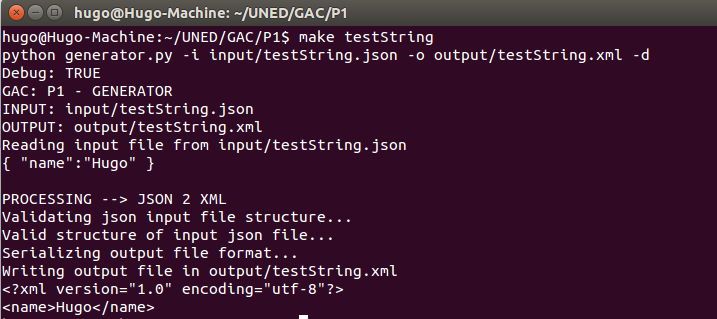
\includegraphics[scale=0.35]{imagenes/testString.png}
\caption{ Test Strings  }  
\end{figure} 

\subsubsection{Numbers}
Tipo de dato: Números

\begin{figure}[H]  
\centering 
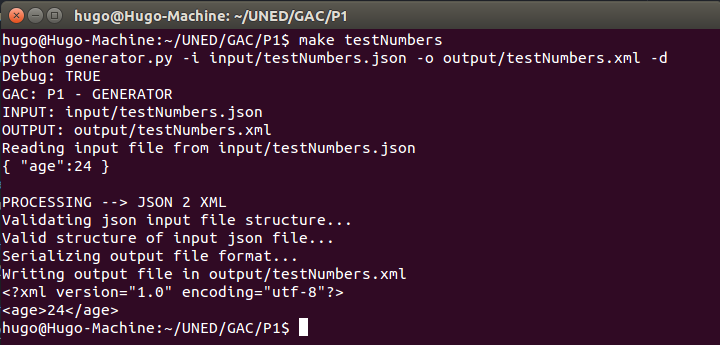
\includegraphics[scale=0.35]{imagenes/testNumbers.png}
\caption{ Test Numbers  }  
\end{figure} 

\subsubsection{Objects}
Tipo de dato: Objetos Json

\begin{figure}[H]  
\centering 
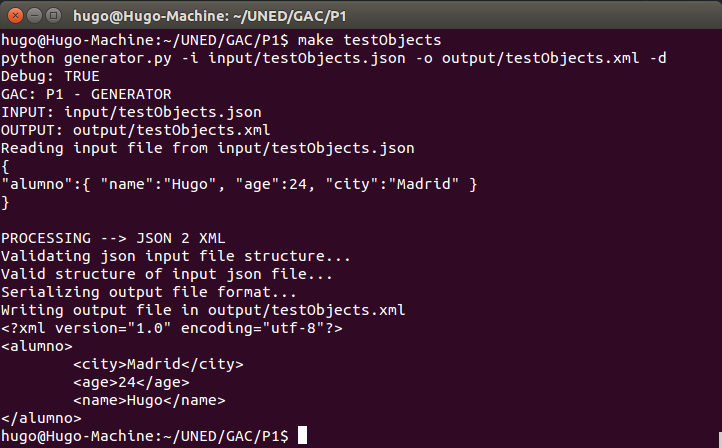
\includegraphics[scale=0.35]{imagenes/testObjects.png}
\caption{ Test Objects  }  
\end{figure} 

\subsubsection{Boolean}
Tipo de dato: Booleanos

\begin{figure}[H]  
\centering 
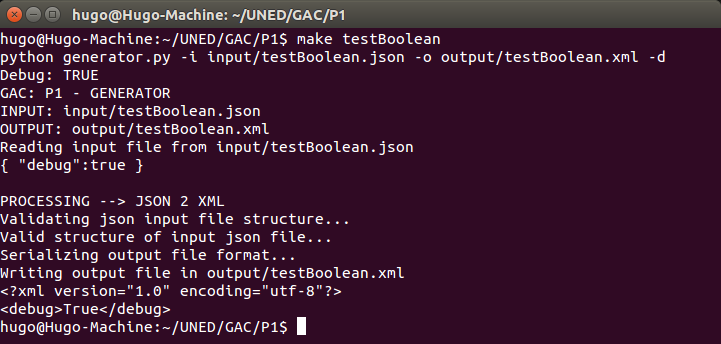
\includegraphics[scale=0.35]{imagenes/testBoolean.png}
\caption{ Test Booleanos  }  
\end{figure} 

\subsubsection{Null}
Tipo de dato: null

\begin{figure}[H]  
\centering 
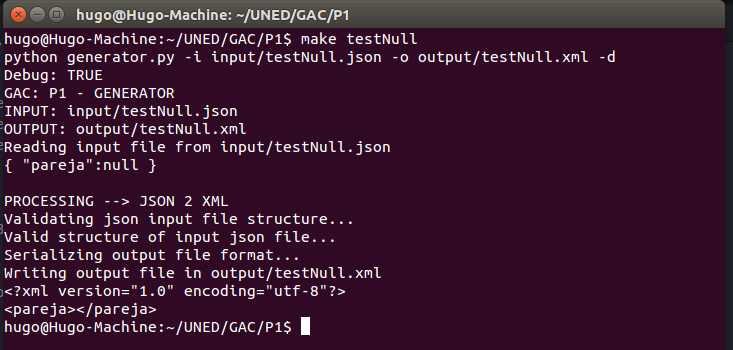
\includegraphics[scale=0.35]{imagenes/testNull.png}
\caption{ Test Null  }  
\end{figure} 

\subsubsection{Arrays}
Tipo de dato: Listas

\begin{figure}[H]  
\centering 
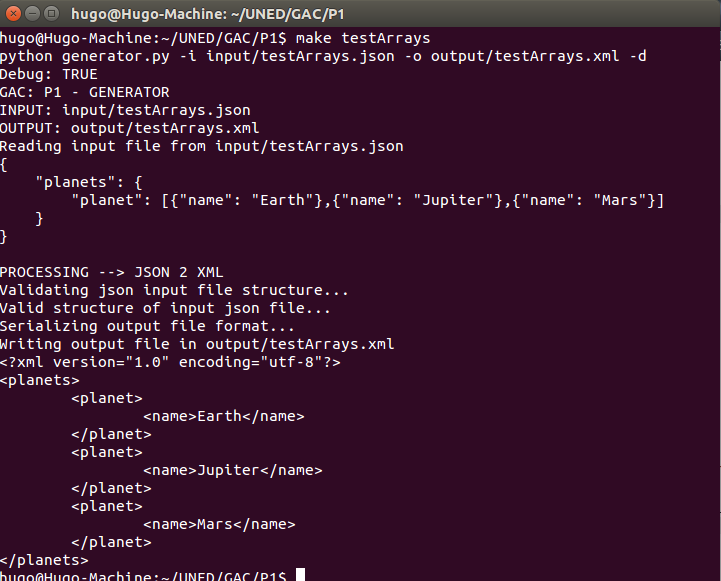
\includegraphics[scale=0.35]{imagenes/testArrays.png}
\caption{ Test Arrays  }  
\end{figure} 

\subsubsection{Json complejos}
La siguiente prueba muestra la capacidad del generador para trabajar con ficheros json complejos, como es por ejemplo el servlet de una aplicación web. Debido a la extensión de la salida de esta prueba, no se adjuntará captura, si no la salida estándar. 
 

\begin{lstlisting}[language=python,caption={make testServlet }]
hugo@Hugo-Machine:~/UNED/GAC/P1$ make testServlet 
python generator.py -i input/servlet.json -o output/output_testservlet.xml -d
Debug: TRUE
GAC: P1 - GENERATOR
INPUT: input/servlet.json
OUTPUT: output/output_testservlet.xml
Reading input file from input/servlet.json
{"web-app": {
  "servlet": [
    {
      "servlet-name": "cofaxCDS",
      "servlet-class": "org.cofax.cds.CDSServlet",
      "init-param": {
        "templateProcessorClass": "org.cofax.WysiwygTemplate",
        "templateLoaderClass": "org.cofax.FilesTemplateLoader",
        "templatePath": "templates",
        "templateOverridePath": "",
        "defaultListTemplate": "listTemplate.htm",
        "defaultFileTemplate": "articleTemplate.htm",
        "useJSP": false,
        "jspListTemplate": "listTemplate.jsp",
        "jspFileTemplate": "articleTemplate.jsp",
        "cachePackageTagsTrack": 200,
        "cachePackageTagsStore": 200,
        "cachePackageTagsRefresh": 60,
        "cacheTemplatesTrack": 100,
        "cacheTemplatesStore": 50,
        "cacheTemplatesRefresh": 15,
        "cachePagesTrack": 200,
        "cachePagesStore": 100,
        "cachePagesRefresh": 10,
        "cachePagesDirtyRead": 10,
        "searchEngineListTemplate": "forSearchEnginesList.htm",
        "searchEngineFileTemplate": "forSearchEngines.htm",
        "searchEngineRobotsDb": "WEB-INF/robots.db",
        "useDataStore": true,
        "dataStoreClass": "org.cofax.SqlDataStore",
        "redirectionClass": "org.cofax.SqlRedirection",
        "dataStoreName": "cofax",
        "dataStoreDriver": "com.microsoft.jdbc.sqlserver.SQLServerDriver",
        "dataStoreUrl": "jdbc:microsoft:sqlserver://LOCALHOST:1433;DatabaseName=goon",
        "dataStoreUser": "sa",
        "dataStorePassword": "dataStoreTestQuery",
        "dataStoreTestQuery": "SET NOCOUNT ON;select test='test';",
        "dataStoreLogFile": "/usr/local/tomcat/logs/datastore.log",
        "dataStoreInitConns": 10,
        "dataStoreMaxConns": 100,
        "dataStoreConnUsageLimit": 100,
        "dataStoreLogLevel": "debug",
        "maxUrlLength": 500}},
    {
      "servlet-name": "cofaxEmail",
      "servlet-class": "org.cofax.cds.EmailServlet",
      "init-param": {
      "mailHost": "mail1",
      "mailHostOverride": "mail2"}},
    {
      "servlet-name": "cofaxAdmin",
      "servlet-class": "org.cofax.cds.AdminServlet"},

    {
      "servlet-name": "fileServlet",
      "servlet-class": "org.cofax.cds.FileServlet"},
    {
      "servlet-name": "cofaxTools",
      "servlet-class": "org.cofax.cms.CofaxToolsServlet",
      "init-param": {
        "templatePath": "toolstemplates/",
        "log": 1,
        "logLocation": "/usr/local/tomcat/logs/CofaxTools.log",
        "logMaxSize": "",
        "dataLog": 1,
        "dataLogLocation": "/usr/local/tomcat/logs/dataLog.log",
        "dataLogMaxSize": "",
        "removePageCache": "/content/admin/remove?cache=pages&id=",
        "removeTemplateCache": "/content/admin/remove?cache=templates&id=",
        "fileTransferFolder": "/usr/local/tomcat/webapps/content/fileTransferFolder",
        "lookInContext": 1,
        "adminGroupID": 4,
        "betaServer": true}}],
  "servlet-mapping": {
    "cofaxCDS": "/",
    "cofaxEmail": "/cofaxutil/aemail/*",
    "cofaxAdmin": "/admin/*",
    "fileServlet": "/static/*",
    "cofaxTools": "/tools/*"},

  "taglib": {
    "taglib-uri": "cofax.tld",
    "taglib-location": "/WEB-INF/tlds/cofax.tld"}}}

PROCESSING --> JSON 2 XML 
Validating json input file structure...
Valid structure of input json file...
Serializing output file format...
Writing output file in output/output_testservlet.xml
<?xml version="1.0" encoding="utf-8"?>
<web-app>
	<servlet-mapping>
		<cofaxTools>/tools/*</cofaxTools>
		<cofaxCDS>/</cofaxCDS>
		<fileServlet>/static/*</fileServlet>
		<cofaxAdmin>/admin/*</cofaxAdmin>
		<cofaxEmail>/cofaxutil/aemail/*</cofaxEmail>
	</servlet-mapping>
	<taglib>
		<taglib-location>/WEB-INF/tlds/cofax.tld</taglib-location>
		<taglib-uri>cofax.tld</taglib-uri>
	</taglib>
	<servlet>
		<servlet-name>cofaxCDS</servlet-name>
		<init-param>
			<cachePagesStore>100</cachePagesStore>
			<searchEngineListTemplate>forSearchEnginesList.htm</searchEngineListTemplate>
			<maxUrlLength>500</maxUrlLength>
			<dataStoreTestQuery>SET NOCOUNT ON;select test='test';</dataStoreTestQuery>
			<defaultFileTemplate>articleTemplate.htm</defaultFileTemplate>
			<dataStoreLogFile>/usr/local/tomcat/logs/datastore.log</dataStoreLogFile>
			<templateLoaderClass>org.cofax.FilesTemplateLoader</templateLoaderClass>
			<dataStoreClass>org.cofax.SqlDataStore</dataStoreClass>
			<templateOverridePath></templateOverridePath>
			<cacheTemplatesStore>50</cacheTemplatesStore>
			<dataStoreUrl>jdbc:microsoft:sqlserver://LOCALHOST:1433;DatabaseName=goon</dataStoreUrl>
			<searchEngineFileTemplate>forSearchEngines.htm</searchEngineFileTemplate>
			<cachePagesTrack>200</cachePagesTrack>
			<cachePackageTagsStore>200</cachePackageTagsStore>
			<dataStoreName>cofax</dataStoreName>
			<dataStorePassword>dataStoreTestQuery</dataStorePassword>
			<useJSP>False</useJSP>
			<defaultListTemplate>listTemplate.htm</defaultListTemplate>
			<dataStoreUser>sa</dataStoreUser>
			<jspListTemplate>listTemplate.jsp</jspListTemplate>
			<jspFileTemplate>articleTemplate.jsp</jspFileTemplate>
			<dataStoreMaxConns>100</dataStoreMaxConns>
			<cachePagesDirtyRead>10</cachePagesDirtyRead>
			<cachePagesRefresh>10</cachePagesRefresh>
			<cacheTemplatesTrack>100</cacheTemplatesTrack>
			<dataStoreConnUsageLimit>100</dataStoreConnUsageLimit>
			<redirectionClass>org.cofax.SqlRedirection</redirectionClass>
			<searchEngineRobotsDb>WEB-INF/robots.db</searchEngineRobotsDb>
			<templateProcessorClass>org.cofax.WysiwygTemplate</templateProcessorClass>
			<cachePackageTagsRefresh>60</cachePackageTagsRefresh>
			<templatePath>templates</templatePath>
			<useDataStore>True</useDataStore>
			<cacheTemplatesRefresh>15</cacheTemplatesRefresh>
			<dataStoreDriver>com.microsoft.jdbc.sqlserver.SQLServerDriver</dataStoreDriver>
			<cachePackageTagsTrack>200</cachePackageTagsTrack>
			<dataStoreLogLevel>debug</dataStoreLogLevel>
			<dataStoreInitConns>10</dataStoreInitConns>
		</init-param>
		<servlet-class>org.cofax.cds.CDSServlet</servlet-class>
	</servlet>
	<servlet>
		<servlet-name>cofaxEmail</servlet-name>
		<init-param>
			<mailHostOverride>mail2</mailHostOverride>
			<mailHost>mail1</mailHost>
		</init-param>
		<servlet-class>org.cofax.cds.EmailServlet</servlet-class>
	</servlet>
	<servlet>
		<servlet-name>cofaxAdmin</servlet-name>
		<servlet-class>org.cofax.cds.AdminServlet</servlet-class>
	</servlet>
	<servlet>
		<servlet-name>fileServlet</servlet-name>
		<servlet-class>org.cofax.cds.FileServlet</servlet-class>
	</servlet>
	<servlet>
		<servlet-name>cofaxTools</servlet-name>
		<init-param>
			<logLocation>/usr/local/tomcat/logs/CofaxTools.log</logLocation>
			<fileTransferFolder>/usr/local/tomcat/webapps/content/fileTransferFolder</fileTransferFolder>
			<log>1</log>
			<dataLog>1</dataLog>
			<dataLogLocation>/usr/local/tomcat/logs/dataLog.log</dataLogLocation>
			<adminGroupID>4</adminGroupID>
			<lookInContext>1</lookInContext>
			<removePageCache>/content/admin/remove?cache=pages&amp;id=</removePageCache>
			<removeTemplateCache>/content/admin/remove?cache=templates&amp;id=</removeTemplateCache>
			<logMaxSize></logMaxSize>
			<dataLogMaxSize></dataLogMaxSize>
			<betaServer>True</betaServer>
			<templatePath>toolstemplates/</templatePath>
		</init-param>
		<servlet-class>org.cofax.cms.CofaxToolsServlet</servlet-class>
	</servlet>
</web-app>
hugo@Hugo-Machine:~/UNED/GAC/P1$
\end{lstlisting}
 
\subsubsection{XML to JSon}
Como parte de la funcionalidad añadida, se va a realizar una unica prueba, en la que el generador va a ingestar un fichero XML y va a generar un fichero JSON.  

\begin{figure}[H]  
\centering 
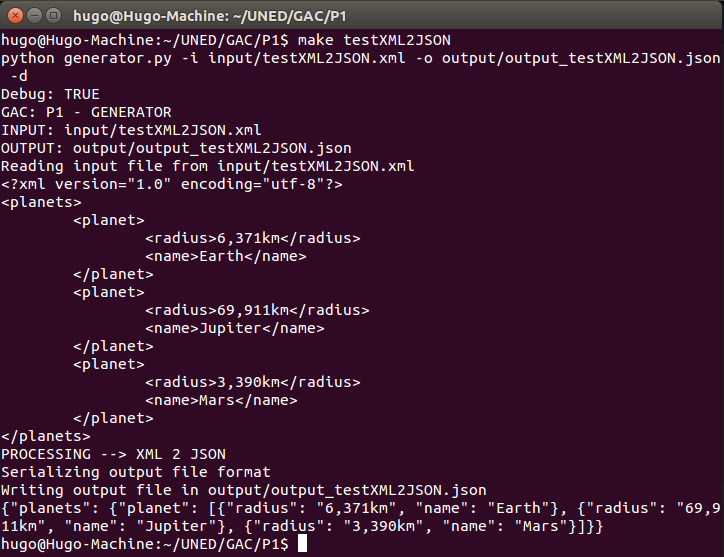
\includegraphics[scale=0.35]{imagenes/testXML2JSON.png}
\caption{ Test XML to Json  }  
\end{figure}
 
\subsection{Pruebas de Error} 

Para realizar las pruebas de error, se ejercitarán los casos en los que las entradas no tengan el formato adecuado o la estructura del json de entrada no sea adecuada.  

\subsubsection{Entrada inexistente}
Si el usuario intenta usar como entrada ficheros que no existen, el generador notificará el error y parará: 

\begin{figure}[H]  
\centering 
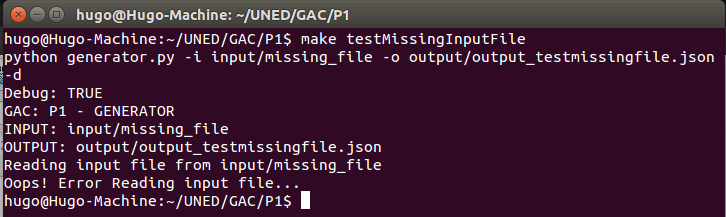
\includegraphics[scale=0.35]{imagenes/missingInput.png}
\caption{ Missing input file  }  
\end{figure}

\subsubsection{Input.format}

Si el usuario del generador intenta usar como entrada ficheros cuya extensión no sea .json o .xml el generador notificará el error y parará: 

\begin{figure}[H]  
\centering 
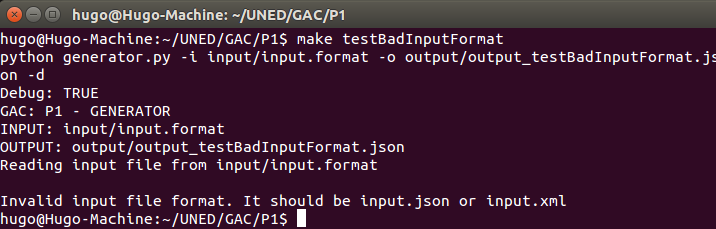
\includegraphics[scale=0.35]{imagenes/badInputFormat.png}
\caption{ Bad input format  }  
\end{figure}

\subsubsection{Estructura Json}

Si el usuario del generador intenta usar como entrada un fichero json cuya estructura no sea la adecuada, el generador notificará el error y parará ya que realiza un chequeo contra esquema solo para los json de entrada. 

\begin{figure}[H]  
\centering 
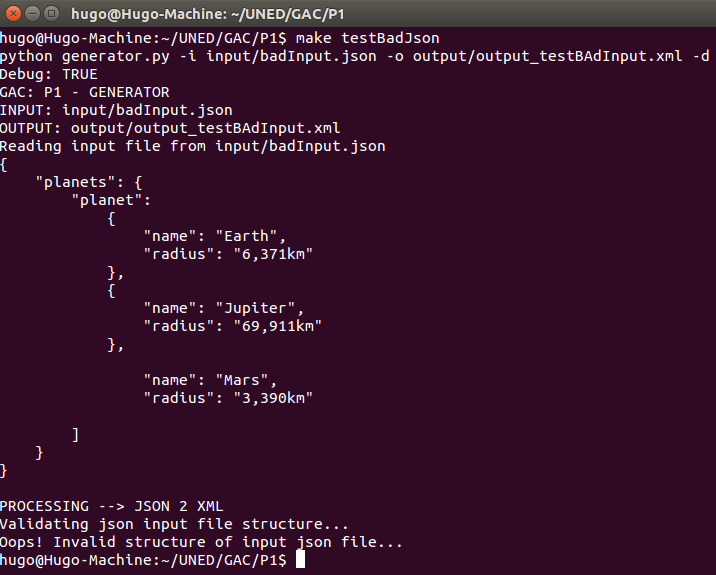
\includegraphics[scale=0.35]{imagenes/badInput.png}
\caption{ Bad input json file  }  
\end{figure}

\chapter{Entrega}
En este capítulo se detallan cada uno de los ficheros/directorios que forman parte de la entrega. 

\section{Generador}
El generador propuesto por el enunciado se compone de un único fichero denominado generator.py el cual se encuentra alojado en la raíz del fichero comprimido que se envía. El generador ha sido desarrollado sobre Ubuntu14 y hace uso de la versión python 2.7.6 la cual incluye todas las dependencias necesarias. Si alguna de ellas causará error, podría ser instalada fácilmente descargando el paquete de las URLs indicadas en la bibliografía y ejecutando sudo pip install nombre\_paquete 

\section{Makefile}
El fichero ''makefile'' establece las distintas ejecuciones de pruebas para el generador. Tambien dispone de la entrada ''make doc'' para generar la especificación software mediante pydoc. Alojado en la raíz del fichero comprimido para la entrega. 

\section{Directorio software specification}
Contiene la especificación del generador en formato HTML. Dicha especificación ha sido generada utilizando la librería pydoc. 

\section{Trabajo1\_CesarHugoBarzanoCruz.pdf}
Memoría de la práctica, referencia a este documento en si mismo, alojado en el directorio raíz de la entrega. 

\section{Directorio DOC}
Directorio donde se almacenan todos los fuentes usados para generar esta documentación utilizando LaTEX. Incluye tambien las imagenes usadas en la memoria. 

\section{Directorio input}
Directorio donde se almacenan todos los ficheros usados como entradas en la sección de pruebas

\section{Directorio Output}
Directorio donde se almacenan todos los ficheros resultados de la ejecución de la pruebas. 

 

\begin{thebibliography}{aaaa}

%intro

\bibitem[1]{xml} \textsc{XML},
\textit{XML Format}
\url{https://www.w3.org/XML/} 


\bibitem[2]{json} \textsc{JSON},
\textit{JSON Format}
\url{https://www.json.org/} 

%Desarrollo

\bibitem[3]{py} \textsc{python},
\textit{Python 2.7.6 language}
\url{https://www.python.org/download/releases/2.7.6/} 


\bibitem[4]{json_lib} \textsc{import json},
\textit{JSON encoder and decoder}
\url{https://docs.python.org/2/library/json.html} 

\bibitem[5]{xmltodic_lib} \textsc{import xmltodic},
\textit{Makes working with XML feel like you are working with JSON}
\url{https://pypi.python.org/pypi/xmltodict} 

\bibitem[6]{sys_lib} \textsc{import sys},
\textit{System-specific parameters and functions}
\url{https://docs.python.org/2/library/sys.html} 

\bibitem[7]{os_lib} \textsc{import os},
\textit{Miscellaneous operating system interfaces}
\url{https://docs.python.org/2/library/os.html} 

\bibitem[8]{getopt_lib} \textsc{import getopt},
\textit{C-style parser for command line options}
\url{https://docs.python.org/2/library/getopt.html}


\end{thebibliography}
 

\chapter{Anexo}
\section{generator.py}
\begin{lstlisting}[language=python,caption={generator.py }]
"""XML generator from file.json"""


__author__ = 'Hugo Barzano'
__date__ = '2017/2018'
__version__ = 'v1.0'
__credits__ = 'GAC'
__file__ = 'generator.py'

import json
import xmltodict
import sys
import os
import getopt

def readInput(input_file):
    """Function to read input files.
         :param input_file: input file path"""
    print "Reading input file from "+input_file
    try:
        with open(input_file, 'r') as f:
    	       input_file_as_string = f.read()
        return input_file_as_string
    except EnvironmentError:
        print("Oops! Error Reading input file...")
        exit()

def writeOutput(output_file,output_string):
    """Function to write output files.
         :param output_file: output file path
         :param output_string: string to write in the output file"""
    print "Writing output file in "+output_file
    try:
        with open(output_file, 'w') as f:
    	       f.write(output_string)
    except EnvironmentError:
        print("Oops! Error writing output file...")
        exit()

def validateJson(input_string):
    """"Function to validate json inputs.
         :param input_string: json as string to validate"""
    try:
        validate_input=json.loads(input_string)
        print "Valid structure of input json file..."
    except ValueError:
        print("Oops! Invalid structure of input json file...")
        exit()

def parseInputJsonToXML(input_string):
    """Function to parse json files as input to XML string.
         :param input_string: input data file as string """
    xmlString = xmltodict.unparse(json.loads(input_string), pretty=True)
    return xmlString

def parseInputXMLToJson(input_string):
    """Function to parse xml files as input to json string.
         :param input_string: input data file as string """
    jsonString = json.dumps(xmltodict.parse(input_string))
    return jsonString

def usage():
    """Method to display generator usage. """
    print """
Usage: python generador.py [options]

Options
-v, --version			Show the version of this script
-h, --help			Show this help.
-i <path>, --input <path>    	Input file
-o <path>, --output <path>     	Output file
-d,         --debug         	Debug Mode
"""

def version():
    """Function to display software version"""
    print "version 1.0"

def main(argv):
    """Main method to execute the generator.
                :param argv: value from 0 to n-1 to ident"""
    input_file=None
    output_file=None
    debug=False

    # process arguments
    try:
        opts, args = getopt.getopt(argv, "hvi:o:d", ["help", "version", "input=","output=","debug"])
    except getopt.GetoptError as err:
        print str(err)
        usage()
        sys.exit(2)
    for opt, arg in opts:
        if opt in ("-h", "--help"):
            usage()
            sys.exit()
        elif opt in ("-v", "--version"):
            version()
            sys.exit()
        elif opt in ("-i", "--input"):
            input_file = arg
        elif opt in ("-o","--output"):
            output_file=arg
        elif opt in ("-d", "--debug"):
            debug = True
            print "Debug: TRUE"
        else:
            usage()
            sys.exit()

    print "GAC: P1 - GENERATOR"
    if debug:
        print "INPUT: "+ input_file
        print "OUTPUT: "+ output_file



    input_as_string=readInput(input_file)
    if debug: print input_as_string
    if input_file.split(".")[1]=="json":
        print "PROCESSING --> JSON 2 XML "
        if debug: print "Validating json input file structure..."
        validateJson(input_as_string)
        if debug: print "Serializing output file format..."
        if not ".xml" in output_file: output_file=output_file+".xml"
        output_as_string=parseInputJsonToXML(input_as_string)
    elif input_file.split(".")[1]=="xml":
        print "PROCESSING --> XML 2 JSON"
        if debug: print "Serializing output file format"
        if not ".json" in output_file: output_file=output_file+".json"
        output_as_string=parseInputXMLToJson(input_as_string)
    else:
        print "Invalid input file format. It should be input.json or input.xml "
        exit()
    writeOutput(output_file,output_as_string)
    if debug:print output_as_string


# --------------------------------------------------------------------------------------------------
# Main exec
# --------------------------------------------------------------------------------------------------

if __name__ == "__main__":
    if len(sys.argv) > 1:
        main(sys.argv[1:])
    else:
        usage()
        sys.exit()

\end{lstlisting}

\section{makefile}
\begin{lstlisting}[language=python,caption={makefile }]
#Makefile

doc:
	rm -r software_specification && mkdir software_specification && pydoc -w ./ && mv ./*.html software_specification/

testString:
	python generator.py -i input/testString.json -o output/testString.xml -d

testNumbers:
	python generator.py -i input/testNumbers.json -o output/testNumbers.xml -d

testObjects:
	python generator.py -i input/testObjects.json -o output/testObjects.xml -d

testBoolean:
		python generator.py -i input/testBoolean.json -o output/testBoolean.xml -d

testNull:
		python generator.py -i input/testNull.json -o output/testNull.xml -d

testArrays:
	python generator.py -i input/testArrays.json -o output/testArrays.xml -d

testServlet:
	python generator.py -i input/servlet.json -o output/output_testservlet.xml -d

testXML2JSON:
		python generator.py -i input/testXML2JSON.xml -o output/output_testXML2JSON.json -d

testBadInputFormat:
		python generator.py -i input/input.format -o output/output_testBadInputFormat.xml -d

testMissingInputFile:
		python generator.py -i input/missing_file -o output/output_testmissingfile.xml -d

testBadJson:
		python generator.py -i input/badInput.json -o output/output_testBAdInput.xml -d

\end{lstlisting}



%
%
%%\nocite{*}
%\bibliography{bibliografia/bibliografia}\addcontentsline{toc}{chapter}{Bibliografía}
%\bibliographystyle{miunsrturl}
%
%\appendix

%\input{apendices/manual_usuario/manual_usuario}
%%\input{apendices/paper/paper}
%\input{glosario/entradas_glosario}
% \addcontentsline{toc}{chapter}{Glosario}
% \printglossary

\thispagestyle{empty}

\end{document}
